\documentclass[spec, och, labwork]{shiza}
% параметр - тип обучения - одно из значений:
%    spec     - специальность
%    bachelor - бакалавриат (по умолчанию)
%    master   - магистратура
% параметр - форма обучения - одно из значений:
%    och   - очное (по умолчанию)
%    zaoch - заочное
% параметр - тип работы - одно из значений:
%    referat    - реферат
%    coursework - курсовая работа (по умолчанию)
%    diploma    - дипломная работа
%    pract      - отчет по практике
% параметр - включение шрифта
%    times    - включение шрифта Times New Roman (если установлен)
%               по умолчанию выключен
\usepackage{subfigure}
\usepackage{tikz,pgfplots}
\pgfplotsset{compat=1.5}
\usepackage{float}

%\usepackage{titlesec}
\setcounter{secnumdepth}{4}
%\titleformat{\paragraph}
%{\normalfont\normalsize}{\theparagraph}{1em}{}
%\titlespacing*{\paragraph}
%{35.5pt}{3.25ex plus 1ex minus .2ex}{1.5ex plus .2ex}

\titleformat{\paragraph}[block]
{\hspace{1.25cm}\normalfont}
{\theparagraph}{1ex}{}
\titlespacing{\paragraph}
{0cm}{2ex plus 1ex minus .2ex}{.4ex plus.2ex}

% --------------------------------------------------------------------------%


\usepackage[T2A]{fontenc}
\usepackage[utf8]{inputenc}
\usepackage{graphicx}
\graphicspath{ {./images/} }
\usepackage{tempora}

\usepackage[sort,compress]{cite}
\usepackage{amsmath}
\usepackage{amssymb}
\usepackage{amsthm}
\usepackage{fancyvrb}
\usepackage{listings}
\usepackage{listingsutf8}
\usepackage{longtable}
\usepackage{array}
\usepackage[english,russian]{babel}

% \usepackage[colorlinks=true]{hyperref}
\usepackage{url}

\usepackage{underscore}
\usepackage{setspace}
\usepackage{indentfirst} 
\usepackage{mathtools}
\usepackage{amsfonts}
\usepackage{enumitem}
\usepackage{tikz}
\usepackage{minted}

\newcommand{\eqdef}{\stackrel {\rm def}{=}}
\newcommand{\specialcell}[2][c]{%
\begin{tabular}[#1]{@{}c@{}}#2\end{tabular}}

\renewcommand\theFancyVerbLine{\small\arabic{FancyVerbLine}}

\newtheorem{lem}{Лемма}

\begin{document}

% Кафедра (в родительном падеже)
\chair{}

% Тема работы
\title{Классификация бинарных отношений и системы замыканий}

% Курс
\course{3}

% Группа
\group{331}

% Факультет (в родительном падеже) (по умолчанию "факультета КНиИТ")
\department{факультета КНиИТ}

% Специальность/направление код - наименование
%\napravlenie{09.03.04 "--- Программная инженерия}
%\napravlenie{010500 "--- Математическое обеспечение и администрирование информационных систем}
%\napravlenie{230100 "--- Информатика и вычислительная техника}
%\napravlenie{231000 "--- Программная инженерия}
\napravlenie{100501 "--- Компьютерная безопасность}

% Для студентки. Для работы студента следующая команда не нужна.
% \studenttitle{Студентки}

% Фамилия, имя, отчество в родительном падеже
\author{Окунькова Сергея Викторовича}

% Заведующий кафедрой
% \chtitle{} % степень, звание
% \chname{}

%Научный руководитель (для реферата преподаватель проверяющий работу)
\satitle{аспирант} %должность, степень, звание
\saname{В. Н. Кутин}

% Руководитель практики от организации (только для практики,
% для остальных типов работ не используется)
% \patitle{к.ф.-м.н.}
% \paname{С.~В.~Миронов}

% Семестр (только для практики, для остальных
% типов работ не используется)
%\term{8}

% Наименование практики (только для практики, для остальных
% типов работ не используется)
%\practtype{преддипломная}

% Продолжительность практики (количество недель) (только для практики,
% для остальных типов работ не используется)
%\duration{4}

% Даты начала и окончания практики (только для практики, для остальных
% типов работ не используется)
%\practStart{30.04.2019}
%\practFinish{27.05.2019}

% Год выполнения отчета
\date{2022}

\maketitle

% Включение нумерации рисунков, формул и таблиц по разделам
% (по умолчанию - нумерация сквозная)
% (допускается оба вида нумерации)
% \secNumbering

%-------------------------------------------------------------------------------------------
\tableofcontents

\section{Постановка задачи}

Цель работы:

Изучение основных свойств бинарных отношений и операций замыкания бинарных отношений.

Порядок выполнения работы:
    \begin{enumerate}
        \item Разобрать основные определения видов бинарных отношений и разработать
        алгоритмы классификации бинарных отношений.
        \item Изучить свойства бинарных отношений и рассмотреть основные системы
        замыкания на множестве бинарных отношений.
        \item Разработать алгоритмы построения основных замыканий бинарных отношений.
    \end{enumerate}

\section{Теоретические сведения по рассмотренным темам с их обоснованием}
        
        Подмножества декартова произведения $A \times B$ множеств $A$ и $B$ называются \textbf{бинарными отношениями} между элементами множеств $A, B$ и обозначаются строчными греческими буквами: $\rho, \sigma, \rho_1, \rho_2, ...$. 

        Для бинарного отношения $\rho \subset A \times B$ область определения $D_\rho$ и множество значений $E_\rho$ определяется как подмножества соответствующих множеств $A$ и $B$ по следующим формулам:

        \[D_\rho = \left\{ a: (a, b) \in \rho \text{ для некоторого } b \in B \right\}\]
        \[E_\rho = \left\{ b: (a, b) \in \rho \text{ для некоторого } a \in A \right\}\]

        Бинарное отношение $\rho \subset A \times A$ является:

        \begin{enumerate}
            \item \textit{рефлексивным}, если $(a, a) \in \rho$ для любого $a \in A$;
            \item \textit{антирефлексивным}, если $(a, a) \notin \rho$ для любого $a \in A$;
            \item \textit{симметричным}, если $(a, b) \in \rho \Rightarrow (b, a) \in \rho$;
            \item \textit{антисимметричным}, если $(a, b) \in \rho \text{ и } (b, a) \in \rho \Rightarrow a = b$;
            \item \textit{транзитивным}, если $(a, b) \in \rho \text{ и } (b, c) \in \rho \Rightarrow (a, c) \in \rho$
            \item \textit{антитранзитивным}, если $(a, b) \in \rho \text{ и } (b, c) \in \rho \Rightarrow (a, c) \notin \rho$
        \end{enumerate}

        Приведем теоретико-множественное истолкование свойств бинарных отношений и перефразируем данное истолкование на язык матриц:
        
        Пусть задано бинарное отношение $\rho \subset A \times A$ и определена матрица данного бинарного отношения $M(\rho)$, тогда бинарное отношение $\rho$ называется

        \begin{enumerate}
            \item \textit{рефлексивным} тогда и только тогда, когда $\Delta_A \subset \rho$. Это означает, что бинарное
            отношение $\rho$ рефлексивно, если $M(\rho) \geq E$, где E - единичная матрица. Если же матрица $M(\rho)$ 
            несравнима с единичной матрицей, то бинарное отношение $\rho$ не является рефлексивным;
            \item \textit{симметричным} тогда и только тогда, когда $\rho^{-1} \subset \rho$. Это означает, что бинарное 
            отношение $\rho$ симметрично, если $M(\rho) \geq M(\rho)^T$, где $M(\rho)^T$ – транспонированная матрица 
            бинарного отношения $\rho$. Если же матрица $M(\rho)$ несравнима с $M(\rho)^T$, то бинарное отношение $\rho$
            не является симметричным;
            \item \textit{транзитивным} тогда и только тогда, когда $\rho \rho \subset \rho$. Это означает, что бинарное
            отношение $\rho$ транзитивно, если $M(\rho)M(\rho) \leq M(\rho)$.
            3. \item \textit{антисимметричным} тогда и только тогда, когда $\rho \cap \rho^{-1} \subset \Delta_A$. Это означает, что бинарное отношение $\rho$ 
            антисимметрично, если $E \geq M(\rho) M(\rho)^T$ (значения элементов вне главной диагонали матрицы $M(\rho) M(\rho)^T$ равны нулю);
        \end{enumerate}

        Классификация бинарных отношений напрямую определяются их свойствами.

        \begin{enumerate}
            \item Рефлексивное транзитивное отношение называется отношением квазипорядка.
            \item Рефлексивное симметричное транзитивное отношение называется отношением эквивалентности.
            \item Рефлексивное антисимметричное транзитивное отношение называется отношением (частичного) порядка.
            \item Антирефлексивное, антисимметричное и транзитивное отношение называется отношением строгого порядка.
        \end{enumerate}

Множество Z подмножеств множества A называется системой замыканий, если оно замкнуто относительно пересечений, т.е. 
выполняется $\cap B \in Z$ для любого подмножества $B \subset Z$.

\textbf{Лемма 1. О системах замыканий бинарных отношений.} 

На множестве $P(A^2)$ всех бинарных отношений между элементами множества A следующие множества являются системами замыканий:

\begin{enumerate}
    \item $Z_r$ - множество всех рефлексивных бинарных отношений между элементами множества A,
    \item $Z_s$ – множество всех симметричных бинарных отношений между элементами множества A,
    \item $Z_t$ – множество всех транзитивных бинарных отношений между элементами множества A,
    \item $Z_{eq} = Eq(A)$ – множество всех отношений эквивалентности на множестве A.
    
\end{enumerate}

Множество $Z_{as}$ всех антисимметричных бинарных отношений между элементами множества A не является системой замыкания.

\textbf{Лемма 2. О замыканиях бинарных отношений.}

На множестве $P(A^2)$ всех бинарных отношений между элементами множества A следующие отображения являются операторами замыканий::

\begin{enumerate}
    \item $f_r (\rho)=\rho \cup \Delta_A$ – наименьшее рефлексивное бинарное отношение, содержащее отношение $\rho \subset A^2$,
    \item $f_s (\rho)= \rho \cup \rho^{-1}$ – наименьшее симметричное бинарное отношение, содержащее отношение $\rho \subset A^2$,
    \item $f_t (\rho)= \cup_{n=1}^\infty \rho^n$  – наименьшее транзитивное бинарное отношение, содержащее отношение $\rho \subset A^2$,
    \item $f_{eq} (\rho)=f_t f_s f_r (\rho)$ – наименьшее отношение эквивалентности, на содержащее отношение $\rho \subset A^2$.
    
\end{enumerate}

\section{Результаты работы}

        \subsection{Описание алгоритма классификации бинарных отношений}
            \begin{enumerate}

                \item Алгоритм 1 - Проверка бинарного отношения на рефлексивность:
                
                Бинарное отношение называется рефлексивным тогда и только тогда, когда $\Delta_A \subset \rho$. Это 
                означает, что бинарное отношение $\rho$ рефлексивно, если $M(\rho) \geq E$, где E - единичная матрица. 
                Если же матрица $M(\rho)$ несравнима с единичной матрицей, то бинарное отношение $\rho$ не является рефлексивным;

                \textit{Вход}: матрица бинарного отношения $A = (a_{ij})$, размерности $n \times n$

                \textit{Выход}: "Множество рефлексивно" или "Множество не рефлексивно"

                Шаг 1. Суммирование элементов на главной диагонали ($sum = \sum\limits_{i=1}^n a[i][i]$). 
                
                Шаг 2. Если $sum = n$, то отношение является рефлексивным, иначе не рефлексивным.

                Асимптотика $O(n)$.

                \item Алгоритм 2 - Проверка бинарного отношения на симметричность:
                
                Бинарное отношение называется симметричным тогда и только тогда, когда $\rho^{-1} \subset \rho$. Это означает, что бинарное 
                отношение $\rho$ симметрично, если $M(\rho) \geq M(\rho)^T$, где $M(\rho)^T$ – транспонированная матрица 
                бинарного отношения $\rho$. Если же матрица $M(\rho)$ несравнима с $M(\rho)^T$, то бинарное отношение $\rho$
                не является симметричным;
                
                \textit{Вход}: матрица бинарного отношения $A = (a_{ij})$, размерности $n \times n$

                \textit{Выход}: "Множество симметрично" или "Множество не симметрично"


                Шаг 1. Транспонируем A, чтобы получить $B = A^T$ ($\forall b[i][j] \in B:$ $b[i][j] = a[j][i]$).

                Шаг 2. Если $A = B$ ($\forall b[i][j] \in B: b[i][j] = a[i][j] $), то бинарное отношение будет является симметричным, иначе отношение не симметрично.

                Асимптотика $O(n^{3/2}logn)$.

                \item Алгоритм 3 - Проверка бинарного отношения на транзитивность:
                
                Бинарное отношение транзитивным тогда и только тогда, когда $\rho \rho \subset \rho$. Это означает, что бинарное
                отношение $\rho$ транзитивно, если $M(\rho)M(\rho) \leq M(\rho)$.
                
                \textit{Вход}: матрица бинарного отношения $A = (a_{ij})$, размерности $n \times n$

                \textit{Выход}: "Множество транзитивно" или "Множество не транзитивно"
                
                На вход подается матрица бинарного отношения A. 
                
                Шаг 1. Получить матрицу $B = A^2$.
                
                Шаг 2. Сравнить полученную и исходную матрицу.
                
                Шаг 3. Если $B \leq A$ ($\forall b[i][j] \in B: b[i][j] \leq a[i][j]$ ), то бинарное отношение транзитивно, иначе не транзитивным.

                Асимптотика $O(n^3)$.

                \item Алгоритм 4 - Проверка бинарного отношения на антирефлексивность:

                \textit{Вход}: матрица бинарного отношения $A = (a_{ij})$, размерности $n \times n$

                \textit{Выход}: "Множество антирефлексивно" или "Множество не антирефлексивно"
                
                На вход подается матрица бинарного отоношения A.

                Шаг 1. Суммирование элементов на главной диагонали ($sum = \sum\limits_{i=1}^n a[i][i]$).
                
                Шаг 2. Если $sum = 0$, то отношение является антирефлексивным, иначе не антирефлексивным.

                Асимптотика $O(n)$.

                \item Алгоритм 5 - Проверка бинарного отношения на антисимметричность:
                
                \textit{Вход}: матрица бинарного отношения $A = (a_{ij})$, размерности $n \times n$

                \textit{Выход}: "Множество антисимметрично" или "Множество не антисимметрично"

                Шаг 1. Транспонируем A, чтобы получить $C = A^T$.

                Шаг 2. Получим матрицу $B = A * C$.

                Шаг 4. Если $ \forall i, j, 0 \leq i, j < n$ $b[i][j]  = 0$, где 
                $b[i][j]$ элемент матрицы B, $i \neq j$, то отношение является антисиметричным, иначе отношение не антисиметрично.

                Асимптотика $O(n^3)$.

                \item Алгоитм 6 - Классификация бинарного отношения:
                
                \textit{Вход}: матрица бинарного отношения $A = (a_{ij})$, размерности $n \times n$

                \textit{Выход}: «Бинарное отношение является отношением квазипорядка», «Бинарное отношение является отношением 
                эквивалентности», «Бинарное отношение является отношением частичного порядка» или «Бинарное отношение 
                является отношением строгого порядка».

                Шаг 1. Запустить алгоритмы 1 и 3 (проверки на рефлексивность и транзитивность), подав им на вход матрицу A. Если алгоритмы вернут значения «Бинарное отношение является рефлексивным» и «Бинарное отношение является транзитивным», то вернуть значение «Бинарное отношение является отношением квазипорядка».

                Шаг 2. Запустить алгоритмы 1, 2 и 3 (проверки на рефлексивность, симметричность и транзитивность), подав им на вход матрицу A. Если алгоритмы вернут значения «Бинарное отношение является рефлексивным», «Бинарное отношение является симметричным» и «Бинарное отношение является транзитивным», то вернуть значение «Бинарное отношение является отношением эквивалентности».

                Шаг 3. Запустить алгоритмы 3 и 5 (проверки на антисимметричность и транзитивность), подав им на вход матрицу A. Если алгоритмы вернут значения «Бинарное отношение является антисимметричным» и «Бинарное отношение является транзитивным», то вернуть значение «Бинарное отношение является отношением частичного порядка».

                Шаг 4. Запустить алгоритмы 3, 4 и 5 (проверки на антирефлексивность, антисимметричность и транзитивность), подав им на вход матрицу A. Если алгоритмы вернут значения «Бинарное отношение является антирефлексивным», «Бинарное отношение является антисимметричным» и Бинарное отношение является транзитивным», то вернуть значение «Бинарное отношение является отношением строгого порядка».

                Если не учитывать сложность вызываемых алгоритмов, то асимптотика $O(1)$, иначе асимптотика $O(n^3)$.

            \end{enumerate}
        
        \subsection{Описание алгоритмов построения основных замыканий бинарных отношений}
            \begin{enumerate}
                
                \item Замыкание бинарного отношения относительно рефлексивности:
                
                \textit{Вход}: матрица бинарного отношения $A = (a_{ij})$, размерности $n \times n$

                \textit{Выход}: матрица бинарного отношения $A'$, замкнутая относительно рефлексивности

                Шаг 1. $\forall i, 0 \leq i < n:$ $a[i][i]$, после чего вернуть полученную матрицу бинарного отношения $A'=(a'_{ij})$ с построенным на нем замыканием рефлексивности.

                Асимптотика $O(n)$.

                \item Замыкание бинарного отношения относительно симметричности:
                
                \textit{Вход}: матрица бинарного отношения $A = (a_{ij})$, размерности $n \times n$

                \textit{Выход}: матрица бинарного отношения $A'$, замкнутая относительно симметричности

                Шаг1. Каждому элементу $a[i][j]$ $0 \leq i, j < n$ матрицы A присваивается значение элемент
                $a[j][i]$, после чего вернуть полученную матрицу бинарного отношения $A'=(a'_{ij})$ с построенным на нем замыканием симметричности.

                Асимптотика $O(n^2)$.

                \item Замыкание бинарного отношения относительно транзитивности:
                
                \textit{Вход}: матрица бинарного отношения $A = (a_{ij})$, размерности $n \times n$

                \textit{Выход}: матрица бинарного отношения $A'$, замкнутая относительно транзитивности

                Шаг1. Если $a[i][k] = 1$ и $a[k][j] = 1$, то установки значения $a[i][j] = 1$, где $0 \leq i,j,k < k$. Такой шаг нужно повторить n раз
                в силу определения п.3) оператора транзитивного замыкания в лемме 2, после чего вернуть полученную матрицу бинарного отношения $A'=(a'_{ij})$ с построенным на нем замыканием транзитивности.

                Асимптотика $O(n^4)$.
            \end{enumerate}
    
        \subsection{Коды программ, реализующей рассмотренные алгоритмы}

            \inputminted[fontsize=\small]{python}{../code/lab1.py}
    
        \subsection{Результаты тестирования программ}

        \begin{figure}[H]
            \centering      %размер рисунка       здесь находится название файла рисунка, без указания формата
            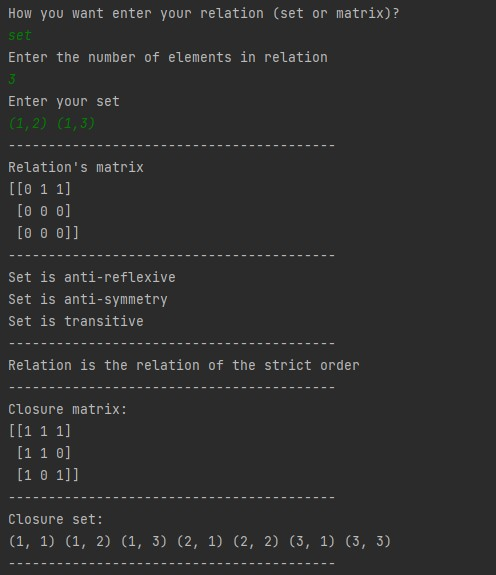
\includegraphics[width=1.\textwidth]{1}
            \caption{Ввод бинарного отношения {(1, 2), (1, 3)} в виде множества с выводом свойств этого множества и замыкания относительно эквивалентности}
            \label{fig:image1}
        \end{figure}
        
        \begin{figure}[H]
            \centering      %размер рисунка       здесь находится название файла рисунка, без указания формата
            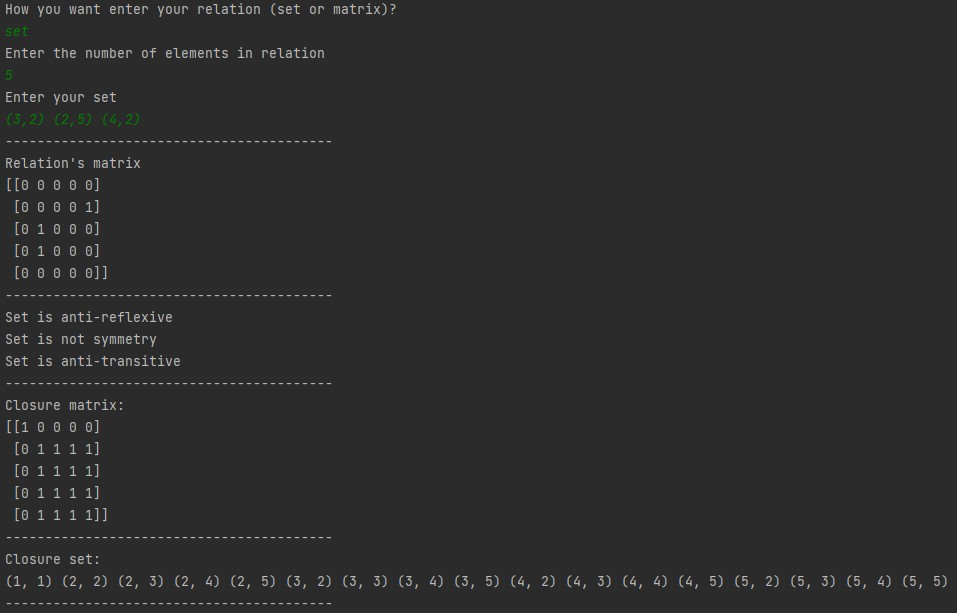
\includegraphics[width=1.\textwidth]{2}
            \caption{Ввод бинарного отношения {(3, 2), (2, 5), (4, 2)} в виде множества с выводом свойств этого множества и замыкания относительно эквивалентности}
            \label{fig:image1}
        \end{figure}

        \begin{figure}[H]
            \centering      %размер рисунка       здесь находится название файла рисунка, без указания формата
            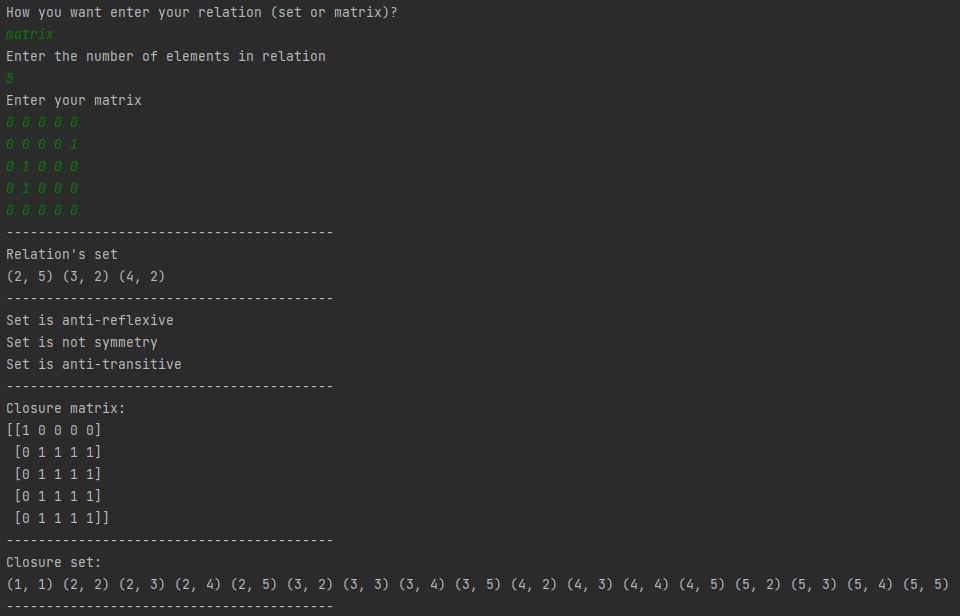
\includegraphics[width=1.\textwidth]{3}
            \caption{Ввод бинарного отношения {(3, 2), (2, 5), (4, 2)} в виде матрицы с выводом свойств этого множества и замыкания относительно эквивалентности}
            \label{fig:image1}
        \end{figure}

        \begin{figure}[H]
            \centering      %размер рисунка       здесь находится название файла рисунка, без указания формата
            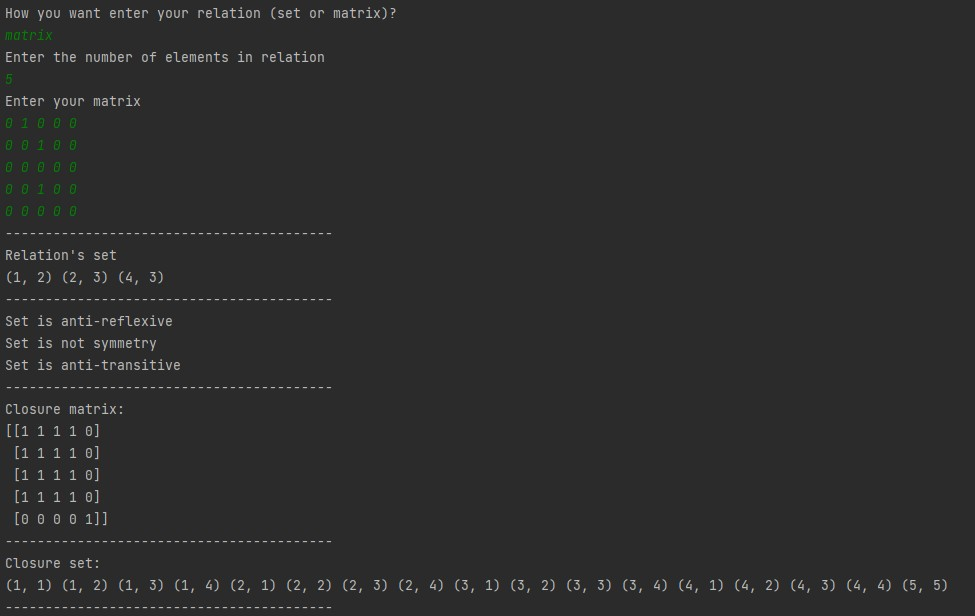
\includegraphics[width=1.\textwidth]{4}
            \caption{Ввод бинарного отношения {(1, 2), (2, 3), (4, 3)} в виде матрицы с выводом свойств этого множества и замыкания относительно эквивалентности}
            \label{fig:image1}
        \end{figure}

        \subsection{Оценки сложности рассмотренных алгоритмов}

        \subsubsection{Алгоритм определения рефлексивности}

            Сложность выполнения проверки на рефлексивность или антирефлексивность определяется как $O(n)$.

        \subsubsection{Алгоритм определения симметричности}

            Cложность транспонирования в numpy определяется как $O(n^{3/2}log \text{ } n)$, сложность умножения матриц 
            определяется как $O(n^3)$, сложность сравнение двух матриц поэлементно определяется как $O(n^2)$. 
            Отсюда можно сделать вывод, что в случае, если наше отношение будет симметричным,
            что будет являтся лучшим случаем раоты алгоритма,то общая сложность алгоритма будет определятся как 
            $O(n^{3/2}log \text{ } n + n^2) = O(n^{3/2}log \text{ } n)$,
            иначе, в худшем случае, сложность будет определятся как $O(n^{3/2}log \text{ } n + n^2 + n^2 + n^3) = O(n^3)$

        \subsubsection{Алгоритм определения транзитивности}

            Из всего выше сказанного очевидно, что сложность проверки на транзитивность или антитранзитивность составляет $O(n^3)$,
            так как в нем используется умножение, сравнение матриц и тройной цикл для проверки рефлексивности в худшем случае матриц.

        \subsubsection{Алгоритм классификации}
            Сложность выполнения самого алгоритма классификации бинарных отношений реализованно через словарь языка python
            и оператор if, поэтому является константной ($O(1)$), если не учитывать сложность выполнения проверки свойств отношения.

        \subsubsection{Построение замыкания рефлексивности}
        
            Так как весь алгоритм строится на заполнении главной диагонали матрицы 1, то его сложность состовляет $O(n)$.

        \subsubsection{Построение замыкания симметричности}

            Для посторения замыкания симметричности используются вложенный цикла, поэтому сложность алгоритма
            определяется как $O(n^2)$.

        \subsubsection{Построение замыкания транзитивности}

            Для посторения замыкания транзитивности используются три вложенный цикла, поэтому сложность алгоритма
            определяется как $O(n^4)$.
    
\conclusion

В рамках данной лабораторной работы были рассмотренны теоритические основы свойств бинарных отношений, их видов и методов
их замыкания по каждому из свойств. На основе этой теоретической части была смоделирована программа на языке Python с 
использованием средств библиотеки Numpy, которая способна определить свойства заданного множества, его вид и построить 
систему замыкания по каждому из основных свойств бинарного отношения, а так же была оценена асимптотика каждого реализованного
алгоритма.

\end{document}
